%
% tikztemplate.tex
%
% (c) 2018 Prof Dr Andreas Müller, Hochschule Rapperswil
%
\documentclass[tikz]{standalone}
\usepackage{times}
\usepackage{amsmath}
\usepackage{txfonts}
\usepackage[utf8]{inputenc}
\usepackage{graphics}
\usepackage{color}
\usepackage{pifont}
\usetikzlibrary{arrows,intersections,math,calc}
\begin{document}

\def\punkt#1{
        \fill[color=white] #1 circle[radius=0.08];
        \draw #1 circle[radius=0.08];
}

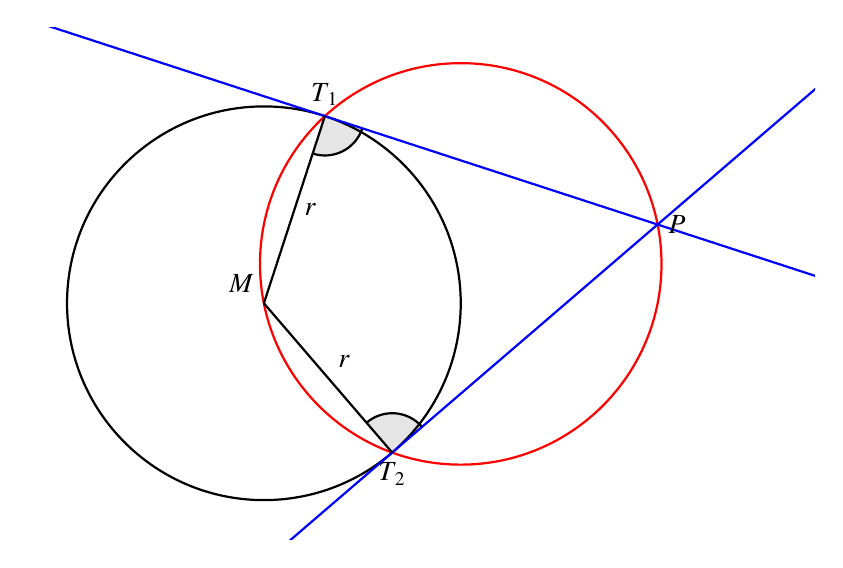
\begin{tikzpicture}[>=latex,thick]

\tikzmath{
	real	\r;
	\r = sqrt(26-(2.5*2.5));
	real	\a, \b;
	\a = atan(2.5 / \r);
	\b = atan(1/5);
}

\coordinate (O) at (0,0);
\coordinate (P) at (5,1);
\coordinate (R) at ({-cos(\a-\b)},{sin(\a-\b)});
\coordinate (V) at ({-cos(\a+\b)},{-sin(\a+\b)});

\coordinate (S) at ($(P)+\r*(R)$);
\coordinate (T) at ($(P)+\r*(V)$);

\fill[color=gray!20] ($(S)-0.5*(R)$) arc ({\b-\a}:{\b-\a-90}:0.5)--(S)--cycle;
\fill[color=gray!20] ($(T)-0.5*(V)$) arc ({\a+\b}:{\a+\b+90}:0.5)--(T)--cycle;
\draw ($(S)-0.5*(R)$) arc ({\b-\a}:{\b-\a-90}:0.5);
\draw ($(T)-0.5*(V)$) arc ({\a+\b}:{\a+\b+90}:0.5);

\draw (0,0) circle[radius=2.5];
\draw[color=red] ($0.5*(P)$) circle[radius={sqrt(26)/2}];

\begin{scope}
\clip (-3,-3) rectangle (7,3.5);
\draw[color=blue] ($(P)-10*(R)$)--($(P)+10*(R)$);
\draw[color=blue] ($(P)-10*(V)$)--($(P)+10*(V)$);
\end{scope}

\node at ($(O)+0.5*(T)$) [above right] {$r$};
\node at ($(O)+0.5*(S)$) [right] {$r$};

\draw (O)--(T);
\draw (O)--(S);

\punkt{(O)} \node at (O) [above left] {$M$};
\punkt{(P)} \node at (P) [right] {$P$};

%\def\punkt#1{
%        \fill[color=white] #1 circle[radius=0.08];
%        \draw[color=blue] #1 circle[radius=0.08];
%}

\punkt{(S)} \node at (S) [above] {$T_1$};
\punkt{(T)} \node at (T) [below] {$T_2$};

\end{tikzpicture}

\end{document}

